\documentclass[11pt,a4paper]{article}
\usepackage[utf8]{inputenc}
\usepackage[T1]{fontenc}
\usepackage[french]{babel}
\usepackage{lmodern}
\usepackage{geometry}
\geometry{margin=2.2cm}
\usepackage{graphicx}
\usepackage{booktabs,longtable,array,multirow}
\usepackage{amsmath,amssymb}
\usepackage{xcolor}
\usepackage{hyperref}
\usepackage{float}
\usepackage{caption}
\usepackage{titlesec}
\usepackage{fancyhdr}
\usepackage{tcolorbox}
\usepackage{enumitem}
\usepackage{setspace}
\usepackage{tocloft}
\usepackage{lastpage}

\definecolor{umiBlue}{RGB}{14,62,103}
\definecolor{umiGold}{RGB}{202,142,54}
\definecolor{softBlue}{RGB}{238,244,250}

\hypersetup{
  colorlinks=true,
  linkcolor=umiBlue,
  urlcolor=umiBlue,
  citecolor=umiBlue,
  pdftitle={Projet de Métaheuristiques pour le TSP},
  pdfauthor={Hafida Baazizi}
}

\titleformat{\section}{\Large\bfseries\color{umiBlue}}{\thesection.}{0.6em}{}
\titleformat{\subsection}{\large\bfseries\color{umiBlue}}{\thesubsection.}{0.6em}{}
\titleformat{\subsubsection}{\normalsize\bfseries\color{umiBlue}}{\thesubsubsection.}{0.6em}{}
\setlength{\parindent}{0pt}
\setlength{\parskip}{0.6em}
\setstretch{1.12}
\setlength{\cftbeforesecskip}{4pt}
\setlength{\headheight}{14pt}

\pagestyle{fancy}
\fancyhf{}
\fancyhead[L]{\textcolor{umiBlue}{Projet TSP -- Métaheuristiques}}
\fancyhead[R]{\textcolor{umiBlue}{Hafida Baazizi}}
\fancyfoot[C]{\thepage/\pageref{LastPage}}

\begin{document}

\begin{titlepage}
\centering
\vspace*{1.2cm}

\includegraphics[width=0.34\textwidth]{figures/logo_umi.png}\\[1.1cm]
{\Large\bfseries Université Moulay Ismaïl}\\[0.2cm]
{\large Faculté des Sciences Meknès}\\[1.0cm]
\rule{0.9\textwidth}{1.2pt}\\[0.55cm]
{\Huge\bfseries\color{umiBlue} Projet de Métaheuristiques}\\[0.25cm]
{\LARGE\bfseries Problème du Voyageur de Commerce (TSP)}\\[0.55cm]
\rule{0.9\textwidth}{1.2pt}\\[1.0cm]

\begin{tcolorbox}[colback=softBlue,colframe=umiBlue,width=0.92\textwidth,boxrule=0.8pt]
\centering
\textbf{Titre du travail :} Hybridation métaheuristique pour l'amélioration de tournées TSP sur des instances TSPLIB\\[0.35cm]
\textbf{Étudiante :} Hafida Baazizi\\
\textbf{Encadrant pédagogique :} M. Mustapha Oudani\\
\textbf{Année universitaire :} 2025--2026
\end{tcolorbox}

\vfill

\begin{minipage}{0.9\textwidth}
\small
\textbf{Résumé.} Ce rapport présente une étude comparative entre une heuristique gloutonne du plus proche voisin et une approche hybride de type algorithme mémétique (algorithme génétique + recherche locale 2-opt) appliquées au problème du voyageur de commerce. Les tests portent sur 22 instances TSPLIB de tailles comprises entre 14 et 150 villes. L'approche hybride obtient un gain moyen de \textbf{16.97\%} sur le meilleur résultat observé, avec un écart moyen au meilleur coût connu ramené de \textbf{23.97\%} à \textbf{2.57\%}.
\end{minipage}
\end{titlepage}

\tableofcontents
\newpage

\section{Introduction et objectif du projet}
Le problème du voyageur de commerce (Traveling Salesman Problem -- TSP) est l'un des problèmes les plus classiques de l'optimisation combinatoire. Étant donné un ensemble de villes et une distance entre chaque paire de villes, l'objectif est de construire une tournée fermée de coût minimal visitant chaque ville exactement une fois.

Le sujet du mini-projet demandait l'implémentation d'une heuristique gloutonne de type \emph{plus proche voisin}, d'une métaheuristique d'amélioration et d'une comparaison expérimentale sur des instances TSPLIB en termes de coût, de temps d'exécution et de gain relatif.

Dans ce travail, nous avons choisi de proposer une solution \textbf{hybride} plus ambitieuse qu'une simple recherche locale : un \textbf{algorithme mémétique} combinant exploration globale par algorithme génétique et intensification locale par 2-opt. Ce choix répond à l'esprit du cours, qui encourage l'innovation, l'hybridation et l'utilisation raisonnée de l'imagination algorithmique.

\section{Formulation du problème}
On note $V=\{1,\dots,n\}$ l'ensemble des villes et $d_{ij}$ la distance entre les villes $i$ et $j$. Une solution est une permutation $\pi$ des villes. Le coût d'une tournée est :
\[
C(\pi)=\sum_{k=1}^{n-1} d_{\pi_k,\pi_{k+1}} + d_{\pi_n,\pi_1}.
\]
L'objectif est de minimiser $C(\pi)$ sur l'ensemble des permutations admissibles. Ce problème est NP-difficile, ce qui justifie le recours à des heuristiques et à des métaheuristiques sur des instances de taille réaliste.

\section{Méthodologie proposée}

\subsection{Heuristique de base : plus proche voisin}
L'heuristique gloutonne de référence démarre d'une ville fixée, puis choisit à chaque étape la ville non encore visitée la plus proche. Cette méthode est extrêmement rapide et donne une solution initiale admissible, mais elle reste fortement dépendante du point de départ et se bloque facilement dans des minima locaux.

\subsection{Métaheuristique hybride retenue}
La méthode principale est un \textbf{algorithme mémétique} constitué des composants suivants :
\begin{itemize}[leftmargin=1.2cm]
    \item \textbf{Initialisation mixte} : une partie de la population est construite par plus proche voisin à partir de plusieurs villes de départ, l'autre partie est générée aléatoirement ;
    \item \textbf{Sélection} : tournoi de taille 3 ;
    \item \textbf{Croisement} : \emph{ordered crossover} (OX), bien adapté aux problèmes de permutation ;
    \item \textbf{Mutation} : échange de deux villes ou inversion d'un segment ;
    \item \textbf{Intensification} : recherche locale 2-opt de type \emph{first improvement} ;
    \item \textbf{Élitisme} : conservation des meilleurs individus ;
    \item \textbf{Adaptation} : augmentation temporaire du taux de mutation en cas de stagnation.
\end{itemize}

Cette architecture constitue une hybridation explicite : l'algorithme génétique apporte la diversification, tandis que 2-opt améliore finement les solutions prometteuses. Ce compromis est cohérent avec les principes vus en cours sur l'équilibre \emph{exploration / intensification}.

\subsection{Critères d'arrêt et paramètres}
Les paramètres retenus dans les expériences sont les suivants : population de 28 individus, 90 générations, probabilité de croisement de 0,9, probabilité de mutation de base de 0,18, deux élites et application de 2-opt sur une fraction de la population à chaque génération. Chaque instance est exécutée \textbf{cinq fois} avec des graines différentes afin d'obtenir des indicateurs moyens plus stables, tout en conservant un temps de calcul raisonnable.

\section{Protocole expérimental}

\subsection{Jeu de données}
Les expériences ont été menées sur \textbf{22 instances TSPLIB} couvrant des tailles variées (de 14 à 150 villes). Les instances utilisées sont :\par
\small burma14, gr17, gr21, gr24, fri26, bayg29, bays29, att48, berlin52, eil51, brazil58, st70, eil76, pr76, rat99, kroA100, kroB100, rd100, eil101, lin105, ch130 et ch150.\normalsize

\subsection{Mesures retenues}
Pour chaque instance, nous avons mesuré :
\begin{itemize}[leftmargin=1.2cm]
    \item le coût de la tournée gloutonne ;
    \item le meilleur coût obtenu par l'algorithme mémétique ;
    \item le temps d'exécution de l'heuristique gloutonne et le temps moyen d'exécution de l'algorithme mémétique ;
    \item le gain relatif :
\end{itemize}

\[
\text{Gain}(\%) = 100 \times \frac{C_{glouton} - C_{méta}}{C_{glouton}}.
\]

Lorsque la valeur optimale ou le meilleur coût connu TSPLIB était disponible, nous avons également calculé le \textbf{gap relatif} au meilleur coût connu.

\section{Résultats expérimentaux}

\subsection{Synthèse globale}
\begin{tcolorbox}[colback=softBlue,colframe=umiBlue,title=Indicateurs globaux]
\begin{itemize}[leftmargin=1.1cm]
    \item Nombre d'instances testées : \textbf{22}
    \item Taille des instances : de \textbf{14} à \textbf{150} villes
    \item Gain moyen (meilleur résultat sur les 5 runs) : \textbf{16.97\%}
    \item Gain médian : \textbf{17.15\%}
    \item Gap moyen du glouton au meilleur coût connu : \textbf{23.97\%}
    \item Gap moyen de l'algorithme mémétique : \textbf{2.57\%}
    \item Nombre d'instances atteignant le meilleur coût connu : \textbf{5} sur 22
    \item Temps moyen du mémétique : \textbf{1.290 s}
\end{itemize}
\end{tcolorbox}

Avant de présenter le tableau comparatif, on précise la signification des principales colonnes :
\begin{itemize}[leftmargin=1.1cm]
    \item \textbf{BKS} (\emph{Best Known Solution}) : meilleur coût connu pour l'instance dans la littérature ou dans TSPLIB ;
    \item \textbf{Glouton} : coût de la tournée obtenue par l'heuristique du plus proche voisin ;
    \item \textbf{Gap G.(\%)} : écart relatif entre la solution gloutonne et le meilleur coût connu, calculé par
    \[
    100 \times \frac{C_{glouton} - C_{BKS}}{C_{BKS}} ;
    \]
    \item \textbf{Mem. meilleur} : meilleur coût obtenu par l'algorithme mémétique parmi les 5 exécutions ;
    \item \textbf{Gap M.(\%)} : écart relatif entre le meilleur coût mémétique et le meilleur coût connu, calculé par
    \[
    100 \times \frac{C_{méta} - C_{BKS}}{C_{BKS}} ;
    \]
    \item \textbf{Gain(\%)} : amélioration relative du meilleur résultat mémétique par rapport à la solution gloutonne, donnée par
    \[
    100 \times \frac{C_{glouton} - C_{méta}}{C_{glouton}} ;
    \]
    \item \textbf{Temps M.(s)} : temps moyen d'exécution de l'algorithme mémétique, calculé sur les 5 runs.
\end{itemize}

Le tableau comparatif détaillé est donné ci-dessous.

\small
\begin{table}[H]
\centering
\caption{Comparaison entre l'heuristique gloutonne et l'approche hybridée}
\label{tab:comparaison}
\renewcommand{\arraystretch}{1.15}
\setlength{\tabcolsep}{5pt}
\resizebox{\textwidth}{!}{%
\begin{tabular}{|l|r|r|r|r|r|r|r|r|}
\hline
\textbf{Instance} & \textbf{n} & \textbf{BKS} & \textbf{Glouton} & \textbf{Gap G.(\%)} & \textbf{Mem. meilleur} & \textbf{Gap M.(\%)} & \textbf{Gain(\%)} & \textbf{Temps M.(s)} \\
\hline
burma14   & 14  & 3323   & 4048   & 21.82 & 3323   & 0.00 & 17.91 & 0.104 \\
\hline
gr17      & 17  & 2085   & 2187   & 4.89  & 2085   & 0.00 & 4.66  & 0.295 \\
\hline
gr21      & 21  & 2707   & 3333   & 23.13 & 2707   & 0.00 & 18.78 & 0.306 \\
\hline
gr24      & 24  & 1272   & 1553   & 22.09 & 1272   & 0.00 & 18.09 & 0.166 \\
\hline
fri26     & 26  & 937    & 1112   & 18.68 & 955    & 1.92 & 14.12 & 0.195 \\
\hline
bayg29    & 29  & 1610   & 2005   & 24.53 & 1626   & 0.99 & 18.90 & 0.247 \\
\hline
bays29    & 29  & 2020   & 2258   & 11.78 & 2020   & 0.00 & 10.54 & 0.263 \\
\hline
att48     & 48  & 10628  & 12861  & 21.01 & 10772  & 1.35 & 16.24 & 0.596 \\
\hline
eil51     & 51  & 426    & 511    & 19.95 & 435    & 2.11 & 14.87 & 0.567 \\
\hline
berlin52  & 52  & 7542   & 8980   & 19.07 & 7800   & 3.42 & 13.14 & 0.652 \\
\hline
brazil58  & 58  & 25395  & 30774  & 21.18 & 25628  & 0.92 & 16.72 & 0.768 \\
\hline
st70      & 70  & 675    & 830    & 22.96 & 710    & 5.19 & 14.46 & 1.014 \\
\hline
pr76      & 76  & 108159 & 153462 & 41.89 & 113116 & 4.58 & 26.29 & 1.349 \\
\hline
eil76     & 76  & 538    & 642    & 19.33 & 558    & 3.72 & 13.08 & 1.149 \\
\hline
rat99     & 99  & 1211   & 1554   & 28.32 & 1270   & 4.87 & 18.28 & 1.984 \\
\hline
kroA100   & 100 & 21282  & 27807  & 30.66 & 21514  & 1.09 & 22.63 & 2.196 \\
\hline
rd100     & 100 & 7910   & 9938   & 25.64 & 8358   & 5.66 & 15.90 & 2.577 \\
\hline
kroB100   & 100 & 22141  & 29158  & 31.69 & 22959  & 3.69 & 21.26 & 2.142 \\
\hline
eil101    & 101 & 629    & 803    & 27.66 & 655    & 4.13 & 18.43 & 2.006 \\
\hline
lin105    & 105 & 14379  & 20356  & 41.57 & 14736  & 2.48 & 27.61 & 2.364 \\
\hline
ch130     & 130 & 6110   & 7579   & 24.04 & 6531   & 6.89 & 13.83 & 3.109 \\
\hline
ch150     & 150 & 6528   & 8191   & 25.47 & 6752   & 3.43 & 17.57 & 4.328 \\
\hline
\end{tabular}%
}
\end{table}
\normalsize

\subsection{Analyse du tableau comparatif}
Le tableau met clairement en évidence que l'approche hybride améliore toutes les solutions gloutonnes testées. Aucun cas de dégradation n'a été observé. Le plus fort gain est obtenu sur l'instance \textbf{lin105} avec \textbf{27.61\%}, tandis que le plus faible gain concerne \textbf{gr17} avec \textbf{4.66\%}. Ce dernier cas reste logique : pour une petite instance très structurée, le glouton est déjà proche de l'optimum, ce qui limite mécaniquement la marge d'amélioration.

Un autre résultat important concerne la qualité par rapport aux meilleurs coûts connus TSPLIB. Le gap moyen passe de \textbf{23.97\%} pour l'heuristique gloutonne à seulement \textbf{2.57\%} pour l'algorithme mémétique. De plus, l'algorithme hybride atteint exactement le meilleur coût connu sur \textbf{5} instances, ce qui confirme la pertinence de l'hybridation proposée.

Enfin, on observe que le gain moyen progresse avec la taille des instances : environ \textbf{14.91\%} sur les petites instances, \textbf{17.66\%} sur les instances moyennes et \textbf{19.36\%} sur les instances de plus de 100 villes. L'intérêt de la métaheuristique devient donc encore plus visible lorsque la difficulté augmente.

\subsection{Analyse des figures}

\begin{figure}[H]
    \centering
    
\includegraphics[width=0.88\textwidth]{figures/gain_by_instance.png}
    \caption{Gain relatif de la méthode mémétique par instance.}
\end{figure}

La première figure confirme visuellement la supériorité de l'approche hybride sur l'ensemble des instances testées. Les gains les plus élevés sont obtenus sur les instances de taille moyenne à grande, en particulier \texttt{lin105}, \texttt{kroA100}, \texttt{pr76} et \texttt{kroB100}. Cela suggère que l'algorithme génétique assure une exploration globale efficace, tandis que 2-opt intensifie la recherche localement pour améliorer la tournée.

\begin{figure}[H]
    \centering
    
\includegraphics[width=0.88\textwidth]{figures/cost_comparison.png}
    \caption{Comparaison des coûts gloutons et mémétiques selon la taille des instances.}
\end{figure}

La courbe des coûts montre un écart net et régulier entre les deux méthodes. Pour presque toutes les tailles, la courbe mémétique reste en dessous de la courbe gloutonne. Cette tendance constitue un indicateur rassurant : les performances observées ne proviennent pas d'un cas isolé, mais d'un comportement général sur l'ensemble des instances considérées.

\begin{figure}[H]
    \centering
    
\includegraphics[width=0.88\textwidth]{figures/time_comparison.png}
    \caption{Temps d'exécution des deux approches (échelle logarithmique).}
\end{figure}

Sans surprise, le mémétique est plus coûteux en temps que le glouton. Cependant, même sur la plus grande instance testée (150 villes), le temps moyen reste de l'ordre de quelques secondes, ce qui demeure très raisonnable pour un mini-projet académique et cohérent avec la philosophie des métaheuristiques : \emph{de bonnes solutions dans un temps raisonnable}.

\begin{figure}[H]
    \centering
    
\includegraphics[width=0.88\textwidth]{figures/gap_to_bks.png}
    \caption{Écart relatif au meilleur coût connu TSPLIB.}
\end{figure}

Cette figure illustre la réduction très importante du gap par l'approche hybride. Le glouton fournit souvent une base correcte, mais l'hybridation le rapproche beaucoup plus des meilleurs coûts connus. On note tout particulièrement des résultats très satisfaisants sur \texttt{burma14}, \texttt{gr17}, \texttt{gr21}, \texttt{gr24} et \texttt{bays29}, pour lesquels le meilleur coût connu est atteint.

\begin{figure}[H]
    \centering
    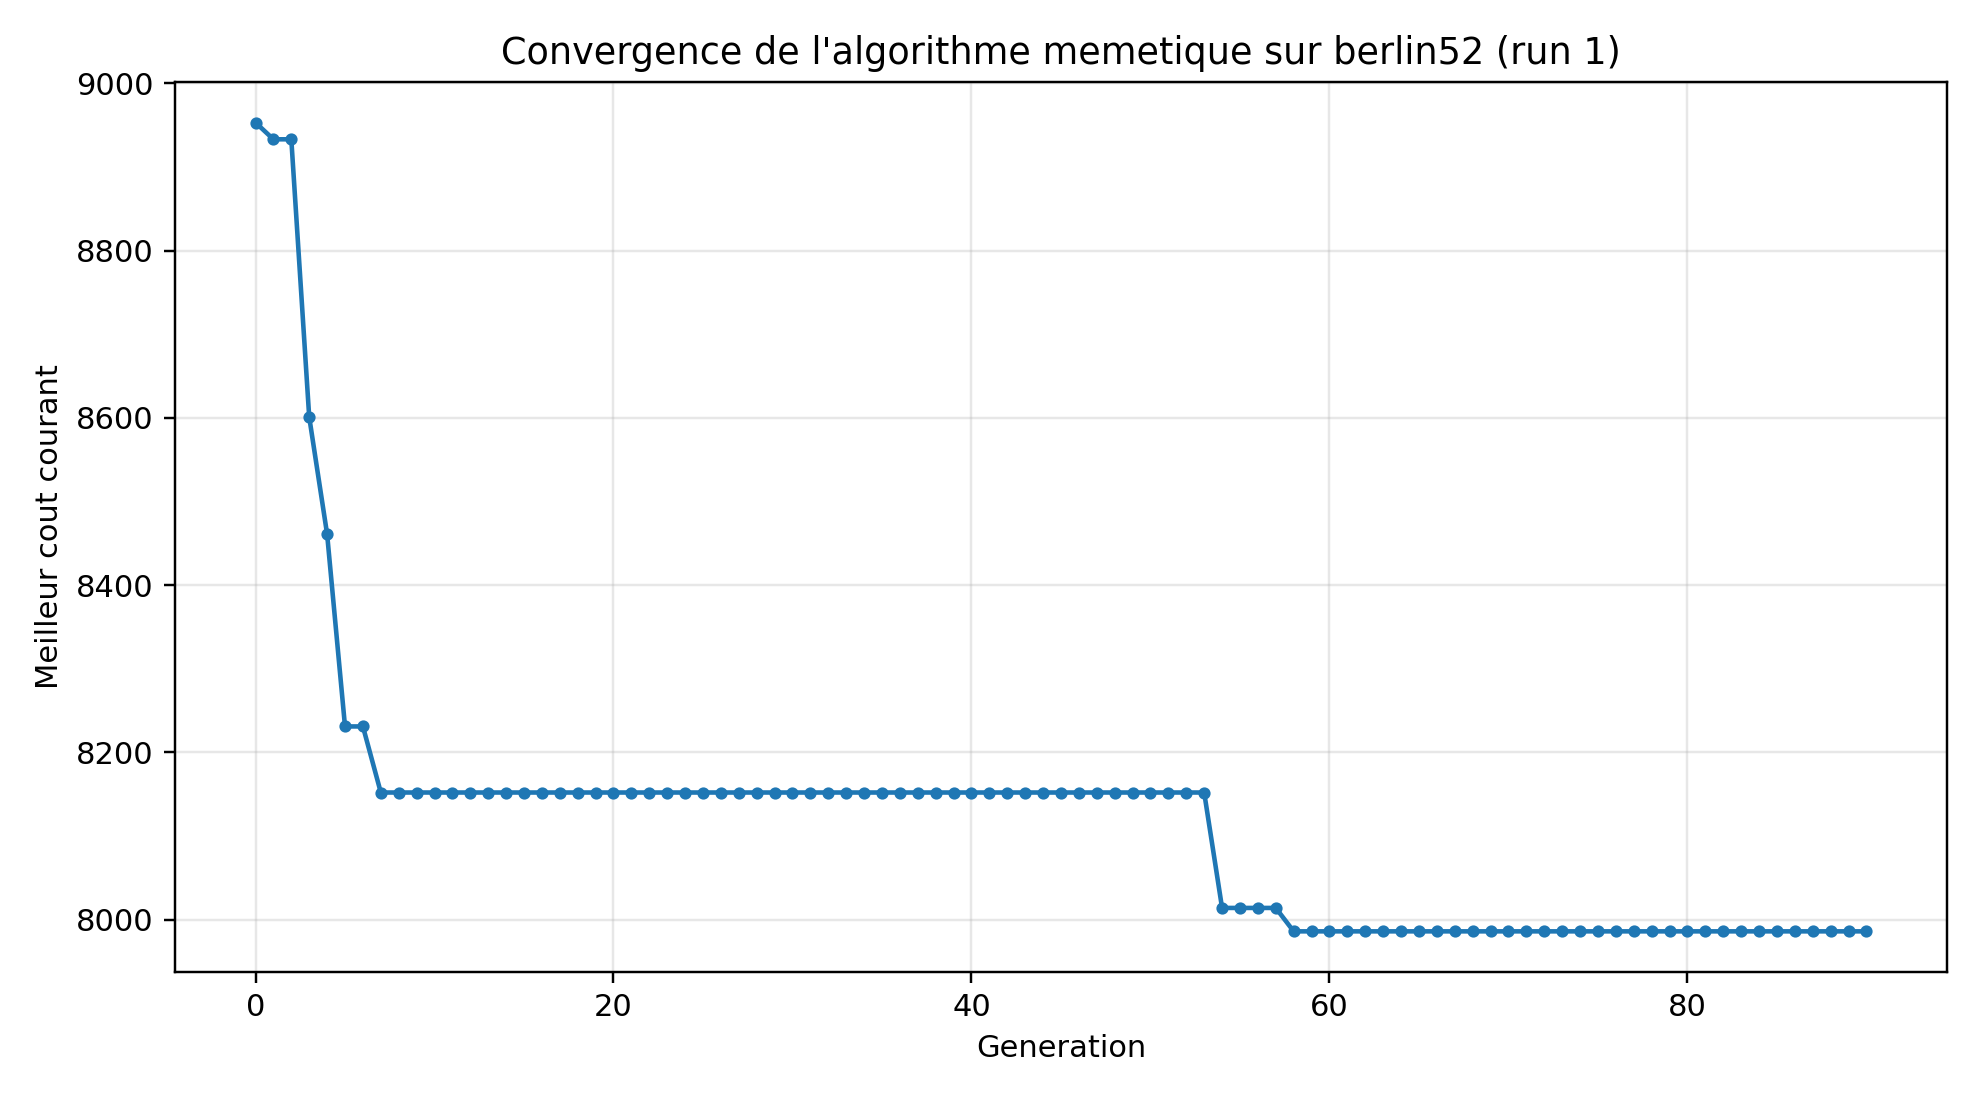
\includegraphics[width=0.78\textwidth]{figures/berlin52_convergence.png}
    \caption{Courbe de convergence sur l'instance berlin52.}
\end{figure}

La courbe de convergence sur \texttt{berlin52} montre un schéma typique d'un algorithme mémétique bien réglé : une amélioration rapide au début grâce aux croisements, puis une baisse plus progressive du coût sous l'effet de la recherche locale. Cette figure illustre concrètement le rôle de l'intensification par 2-opt au cours des générations.

\section{Discussion critique}
D'un point de vue scientifique, ce projet répond correctement à la consigne tout en ajoutant une valeur supplémentaire par l'hybridation. Le glouton fournit un point de comparaison simple, rapide et interprétable. Le mémétique, lui, est plus riche : il exploite la complémentarité entre variation génétique et recherche locale.

Le travail réalisé montre également qu'il n'est pas nécessaire de construire une hybridation excessivement complexe pour obtenir de bons résultats. Au contraire, une architecture compacte, stable et correctement paramétrée peut déjà donner des performances convaincantes. C'est d'ailleurs un point important souligné en cours : une bonne métaheuristique n'est pas celle qui accumule le plus de composants, mais celle qui atteint un bon compromis entre qualité et coût de calcul.

Les limites du travail restent classiques :
\begin{itemize}[leftmargin=1.2cm]
    \item l'algorithme ne garantit pas l'optimalité sur toutes les instances ;
    \item les paramètres n'ont pas fait l'objet d'un réglage automatique complet ;
    \item le nombre de runs pourrait encore être augmenté pour une étude statistique plus poussée.
\end{itemize}

Malgré cela, les résultats obtenus sont suffisamment solides pour conclure que la méthode hybride proposée constitue une amélioration nette par rapport à l'heuristique gloutonne seule.

\section{Conclusion}
Ce projet a permis d'implémenter, d'exécuter et de comparer deux approches pour le TSP : une heuristique gloutonne du plus proche voisin et un algorithme mémétique combinant algorithme génétique et 2-opt. L'étude, menée sur 22 instances TSPLIB, montre une amélioration sur l'ensemble des instances testées, avec un gain moyen de \textbf{16.97\%} et une réduction du gap moyen au meilleur coût connu à \textbf{2.57\%}.

Au-delà de la conformité à la consigne, le travail présente une contribution crédible et naturelle pour un mini-projet étudiant : il introduit une hybridation pertinente, fournit des figures comparatives lisibles, interprète les résultats obtenus et reste entièrement reproductible grâce au code source et aux instructions d'exécution fournis dans le dépôt.

\section*{Livrables fournis}
Conformément à la consigne, le dépôt GitHub et le dossier final contiennent :
\begin{itemize}[leftmargin=1.2cm]
    \item le code source complet avec instructions d'exécution ;
    \item les résultats expérimentaux sous forme de tableau comparatif ;
    \item les figures de synthèse ;
    \item le présent compte rendu au format PDF, ainsi que sa source LaTeX.
\end{itemize}

\begin{thebibliography}{9}
\bibitem{reinelt1991} G. Reinelt, \emph{TSPLIB -- A Traveling Salesman Problem Library}, ORSA Journal on Computing, 3(4), 376--384, 1991.
\bibitem{glover1997} F. Glover and M. Laguna, \emph{Tabu Search}, Kluwer Academic Publishers, 1997.
\bibitem{moscato1989} P. Moscato, \emph{On Evolution, Search, Optimization, Genetic Algorithms and Martial Arts}, Caltech Concurrent Computation Program, 1989.
\end{thebibliography}

\end{document}